\documentclass{article}
\usepackage[utf8]{inputenc}
\usepackage{graphicx}% http://ctan.org/pkg/graphicx
\usepackage[ngerman]{babel}
\usepackage{float}
\usepackage{fancyhdr}
\usepackage{geometry}
\usepackage{hyperref}
\geometry{a4paper, left=30mm, right=20mm,top=25mm,bottom=25mm}
	\fancyhead{}
	%Kopfzeile links
	\fancyhead[L]{Softwareprojetkt WS 2018/19 - SS2018\\Technologierecherche}
	%Kopfzeile rechts
	\fancyhead[R]{HTWK Leipzig, IMN \\ Gruppe 7}
	
\begin{document}
\pagestyle{fancy}

\section{Aufgabe: GUI-Frameworks (4)}

Untersuche die Folgenden Frameworks zur Entwicklung einer grafischen Benutzeroberfläche in Python:
\begin{enumerate}
    \item pyGTK mit Glade
    \item Tkinter
    \item PyGUI
    \item libavg
    \item PyGObject
    \item Pyforms
    \item PyQt5 mit QtCreator
    \item wxWidgets
\end{enumerate}
Betrachte dabei unterem Anderem:
\begin{itemize}
    \item Stärken und Schwächen
    \item Plattformunabhängigkeit
    \item Videodarstellung
    \item Qualität der Dokumentation
    \item Schwierigkeitsgrad der Benutzung
    \item Lernbarkeit
    \item Maintenance
    \item Lizenz (academic/commercial use)
    \item Anpassbarkeit (eigene Widgets)
    \item Python3 Unterstützung
\end{itemize}
Erstelle die in der Abbildung \ref{fig:my_label} dargestellte GUI möglichst Detail getreu mit jedem Framework in beiden Designs und vergleiche die Handhabung.
\begin{figure}[H]
    \centering
    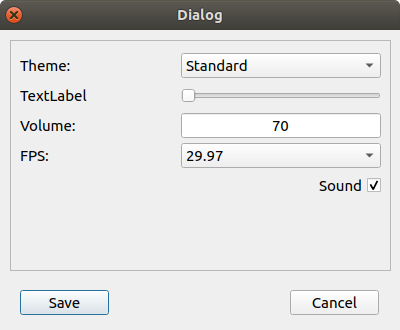
\includegraphics[width=6cm]{technologierecherche/TestGui-light.png}\hspace{1cm}
    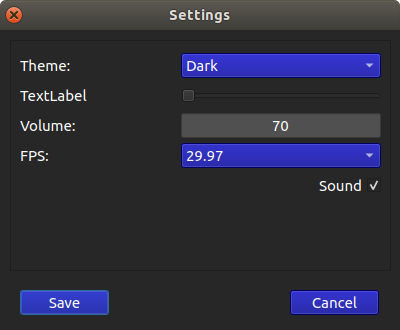
\includegraphics[width=6cm]{technologierecherche/TestGui-dark.png}
    \caption{Test-GUI in hellem und dunkelem Design}
    \label{fig:my_label}
\end{figure}
\textbf{Ansprechpartner:}
\\\\
Tim Jeske (\emph{Softwarearchitekt}), tim.jeske@stud.htwk-leipzig.de

\newpage

\section{Aufgabe: Videoediting (1)}
Untersuche das Videoediting Python Module MoviePy auf:
\begin{itemize}
    \item Eignung für das Projekt
    \item Rendering und Export von Videos
    \item Qualität der Dokumentation
    \item Benutzung für Videos und andere Mediendateien (Bild, PDF, Ton)
    \item Schwierigkeitsgrad der Benutzung
    \item Maintenance
    \item Lizenz (academic/commercial use)
    \item Python3 Unterstützung
\end{itemize}
Suche nach alternativen Videomodulen und vergleiche diese mit MoviePy (evtl. OpenShot Library).
\\\\
\textbf{Ansprechpartner:}
\\\\
Tim Jeske (\emph{Softwarearchitekt}), tim.jeske@stud.htwk-leipzig.de

\newpage

\section{Aufgabe: OpenCV (1)}
Untersuche die Bibliothek OpenCV und erläutere Benutzung und Möglichkeiten. Untersuche die Eignung dieser Bibliothek für unser Projekt und finde gegebenenfalls Alternativen.
Finde heraus, ob OpenCV kompiliert werden muss und wie man es in einem Projekt einbindet, sodass es auf unterschiedlichen Betriebssystemen funktioniert (Linux, Windows, Mac).
\\\\
Untersuche NumPy und beschreibe den Nutzen dieser Bibliothek. Erläutere die Verwendung und die Vor- und Nachteile der Bibliothek.
\\\\
\textbf{Ansprechpartner:}
\\\\
Tim Jeske (\emph{Softwarearchitekt}), tim.jeske@stud.htwk-leipzig.de
\newpage

\section{Aufgabe: Face-Tracking (2)}
Untersuche verschiedene Face Tracking Methoden (z.B. Haar, LBP) auf ihre Eignung für das Projekt. Gehe dabei möglichst auf folgende Punkte ein:
\begin{itemize}
    \item Sidedetection
    \item maximale Entfernung zur Kamera
    \item Voraussetzungen
    \item minimale Auflösung
    \item Ausgabedaten
    \item Ressourcenverbrauch
    \item Echtzeitfähigkeit
    \item Sind Trainingsdaten erforderlich?
    \item Bestehende, nutzbare Implementierungen
    \item Qualität (Sensibilität und Entstehung von Ghosts)
\end{itemize}
\textbf{Ansprechpartner:}
\\\\
Tim Jeske (\emph{Softwarearchitekt}), tim.jeske@stud.htwk-leipzig.de

\newpage
\section{Aufgabe: Face-Tracking-Bibliotheken (1)}
Untersuche die API \href{https://github.com/ageitgey/face\_recognition}{Face Recognition} und die API \href{https://github.com/cmusatyalab/openface}{Openface} auf:
\begin{itemize}
    \item Eignung für das Projekt
    \item Verwendete Methode zur Gesichtserkennung
    \item Voraussetzungen
    \item Qualität der Gesichtserkennung
    \item Qualität der Dokumentation
    \item Schwierigkeitsgrad der Benutzung
    \item Maintenance
    \item Ausgabedaten
    \item Lizenz (academic/commercial use)
    \item Plattformunabhängigkeit
    \item Python3 Unterstützung
\end{itemize}
\textbf{Ansprechpartner:}
\\\\
Tim Jeske (\emph{Softwarearchitekt}), tim.jeske@stud.htwk-leipzig.de

\newpage

\section{Aufgabe: PDF-Konverter (1)}
Untersuche, wie PDF-Dateien mit Python in Bilder und andere Formate konvertiert werden können.\\
Betrachte und Vergleiche dabei diese Bibliotheken:
\begin{enumerate}
    \item \href{https://gitlab.com/pdftools/python-ghostscript}{Ghostscript}
    \item \href{http://www.imagemagick.org/script/index.php}{ImageMagick}
\end{enumerate}
Untersuche dabei auch:
\begin{itemize}
    \item Benutzung
    \item Plattformunabhängigkeit
    \item Python3 Unterstützung
    \item Größe der Bibliothek
    \item Maintenance
\end{itemize}
Finde gegebenenfalls Alternativen und vergleiche diese mit den oben genannten Bibliotheken.

\section{Aufgabe: Benutzereinstellungen (1)}\label{sec:usersettings}
Untersuche wie Einstellungen eines Benutzers gespeichert werden können. Betrachte dabei die Dateiformate ini, json und yaml und die Bibliotheken:
\begin{enumerate}
    \item ConfigParser
    \item PyYaml
    \item json
\end{enumerate}
Eine ausführliche Erläuterung des Themas findest du hier:\\ \url{https://pyvideo.org/pycon-us-2009/pycon-2009--data-storage-in-python---an-overview0.html}
\\\\
\textbf{Ansprechpartner:}
\\\\
Tim Jeske (\emph{Softwarearchitekt}), tim.jeske@stud.htwk-leipzig.de

\newpage

\section{Aufgabe: Cross-Plattform-Deployment von Python (1)}
Untersuche wie ein Python Projekt auf Windows und auf Linux deployed werden kann.\\
Untersuche dabei die Module:
\begin{enumerate}
    \item Pyinstaller
    \item fbs
    \item cx\_freeze
\end{enumerate}
Suche nach Alternativen und vergleiche diese gegebenenfalls mit den oben genannten Modulen. Erfüllen diese Frameworks die Anforderungen:
\begin{itemize}
    \item Windows und Linux Excecutable
    \item mit OpenCV
    \item mit GUI, wie PyQt
    \item Config-Dateien nach Freeze benutzbar (vergleiche Aufgabe \ref{sec:usersettings})
Zum Test deploye deine Programmieraufgabe oder die Vorlage der Programmieraufgabe für Windows und für Linux. Gibt es bestimmte Vorraussetzungen, die erfüllt sein müssen, damit ein Projekt gefreezed werden kann?
\end{itemize}
\textbf{Ansprechpartner:}
\\\\
Tim Jeske (\emph{Softwarearchitekt}), tim.jeske@stud.htwk-leipzig.de
\end{document}
